%!TEX TS-program = xelatex

% Шаблон документа LaTeX создан в 2018 году
% Алексеем Подчезерцевым
% В качестве исходных использованы шаблоны
% 	Данилом Фёдоровых (danil@fedorovykh.ru) 
%		https://www.writelatex.com/coursera/latex/5.2.2
%	LaTeX-шаблон для русской кандидатской диссертации и её автореферата.
%		https://github.com/AndreyAkinshin/Russian-Phd-LaTeX-Dissertation-Template

\documentclass[a4paper,14pt]{article}


%%% Работа с русским языком
\usepackage[english,russian]{babel}   %% загружает пакет многоязыковой вёрстки
\usepackage{fontspec}      %% подготавливает загрузку шрифтов Open Type, True Type и др.
\defaultfontfeatures{Ligatures={TeX},Renderer=Basic}  %% свойства шрифтов по умолчанию
\setmainfont[Ligatures={TeX,Historic}]{Times New Roman} %% задаёт основной шрифт документа
\setsansfont{Comic Sans MS}                    %% задаёт шрифт без засечек
\setmonofont{Courier New}
\usepackage{indentfirst}
\frenchspacing

\renewcommand{\epsilon}{\ensuremath{\varepsilon}}
\renewcommand{\phi}{\ensuremath{\varphi}}
\renewcommand{\kappa}{\ensuremath{\varkappa}}
\renewcommand{\le}{\ensuremath{\leqslant}}
\renewcommand{\leq}{\ensuremath{\leqslant}}
\renewcommand{\ge}{\ensuremath{\geqslant}}
\renewcommand{\geq}{\ensuremath{\geqslant}}
\renewcommand{\emptyset}{\varnothing}

%%% Дополнительная работа с математикой
\usepackage{amsmath,amsfonts,amssymb,amsthm,mathtools} % AMS
\usepackage{icomma} % "Умная" запятая: $0,2$ --- число, $0, 2$ --- перечисление

%% Номера формул
%\mathtoolsset{showonlyrefs=true} % Показывать номера только у тех формул, на которые есть \eqref{} в тексте.
%\usepackage{leqno} % Нумерация формул слева	

%% Перенос знаков в формулах (по Львовскому)
\newcommand*{\hm}[1]{#1\nobreak\discretionary{}
	{\hbox{$\mathsurround=0pt #1$}}{}}

%%% Работа с картинками
\usepackage{graphicx}  % Для вставки рисунков
\graphicspath{{images/}}  % папки с картинками
\setlength\fboxsep{3pt} % Отступ рамки \fbox{} от рисунка
\setlength\fboxrule{1pt} % Толщина линий рамки \fbox{}
\usepackage{wrapfig} % Обтекание рисунков текстом

%%% Работа с таблицами
\usepackage{array,tabularx,tabulary,booktabs} % Дополнительная работа с таблицами
\usepackage{longtable}  % Длинные таблицы
\usepackage{multirow} % Слияние строк в таблице
\usepackage{float}% http://ctan.org/pkg/float

%%% Программирование
\usepackage{etoolbox} % логические операторы


%%% Страница
\usepackage{extsizes} % Возможность сделать 14-й шрифт
\usepackage{geometry} % Простой способ задавать поля
\geometry{top=20mm}
\geometry{bottom=20mm}
\geometry{left=20mm}
\geometry{right=10mm}
%
%\usepackage{fancyhdr} % Колонтитулы
% 	\pagestyle{fancy}
%\renewcommand{\headrulewidth}{0pt}  % Толщина линейки, отчеркивающей верхний колонтитул
% 	\lfoot{Нижний левый}
% 	\rfoot{Нижний правый}
% 	\rhead{Верхний правый}
% 	\chead{Верхний в центре}
% 	\lhead{Верхний левый}
%	\cfoot{Нижний в центре} % По умолчанию здесь номер страницы

\usepackage{setspace} % Интерлиньяж
\onehalfspacing % Интерлиньяж 1.5
%\doublespacing % Интерлиньяж 2
%\singlespacing % Интерлиньяж 1

\usepackage{lastpage} % Узнать, сколько всего страниц в документе.

\usepackage{soul} % Модификаторы начертания

\usepackage{hyperref}
\usepackage[usenames,dvipsnames,svgnames,table,rgb]{xcolor}
\hypersetup{				% Гиперссылки
	unicode=true,           % русские буквы в раздела PDF
	pdftitle={Практическая по БД},   % Заголовок
	pdfauthor={Подчезерцев Алексей},      % Автор
	pdfsubject={Создание и заполнение отношений БД фитнес-клуба},      % Тема
	pdfcreator={Подчезерцев Алексей}, % Создатель
	pdfproducer={Подчезерцев Алексей}, % Производитель
	pdfkeywords={БД} {SQL} {MySQL}, % Ключевые слова
	colorlinks=true,       	% false: ссылки в рамках; true: цветные ссылки
	linkcolor=black,          % внутренние ссылки
	citecolor=black,        % на библиографию
	filecolor=magenta,      % на файлы
	urlcolor=black           % на URL
}
\makeatletter 
\def\@biblabel#1{#1. } 
\makeatother
\usepackage{cite} % Работа с библиографией
%\usepackage[superscript]{cite} % Ссылки в верхних индексах
%\usepackage[nocompress]{cite} % 
\usepackage{csquotes} % Еще инструменты для ссылок

\usepackage{multicol} % Несколько колонок

\usepackage{tikz} % Работа с графикой
\usepackage{pgfplots}
\usepackage{pgfplotstable}

% ГОСТ заголовки
\usepackage[font=small]{caption}
%\captionsetup[table]{justification=centering, labelsep = newline} % Таблицы по правобу краю
%\captionsetup[figure]{justification=centering} % Картинки по центру


\newcommand{\tablecaption}[1]{\addtocounter{table}{1}\small \begin{flushright}\tablename \ \thetable\end{flushright}%	
\begin{center}#1\end{center}}

\newcommand{\imref}[1]{Рис.~\ref{#1}}

\usepackage{multirow}
\usepackage{spreadtab}
\newcolumntype{K}[1]{@{}>{\centering\arraybackslash}p{#1cm}@{}}


\usepackage{xparse}
\ExplSyntaxOn
\DeclareExpandableDocumentCommand{\juliandate}{ m m m }
{
	\juliandate_calc:nnnn { #1 } { #2 } { #3 } { \use:n }
}
\NewDocumentCommand{\storejuliandate}{ s m m m m }
{
	\IfBooleanTF{#1}
	{
		\juliandate_calc:nnnn { #3 } { #4 } { #5 } { \cs_set:Npx #2 }
	}
	{
		\juliandate_calc:nnnn { #3 } { #4 } { #5 } { \cs_new:Npx #2 }
	}
}
\cs_new:Npn \juliandate_calc:nnnn #1 #2 #3 #4 % #1 = day, #2 = month, #3 = year, #4 = what to do
{
	#4 
	{
		\int_eval:n
		{
			#1 +
			\int_div_truncate:nn { 153 * (#2 + 12 * \int_div_truncate:nn { 14 - #2 } { 12 } - 3) + 2 } { 5 } +
			365 * (#3 + 4800 - \int_div_truncate:nn { 14 - #2 } { 12 } ) +
			\int_div_truncate:nn { #3 + 4800 - \int_div_truncate:nn { 14 - #2 } { 12 } } { 4 } -
			\int_div_truncate:nn { #3 + 4800 - \int_div_truncate:nn { 14 - #2 } { 12 } } { 100 } + 
			\int_div_truncate:nn { #3 + 4800 - \int_div_truncate:nn { 14 - #2 } { 12 } } { 400 } -
			32045
		}
	}
}

\tl_new:N \l__juliandate_g_tl
\tl_new:N \l__juliandate_dg_tl
\tl_new:N \l__juliandate_c_tl
\tl_new:N \l__juliandate_dc_tl
\tl_new:N \l__juliandate_b_tl
\tl_new:N \l__juliandate_db_tl
\tl_new:N \l__juliandate_a_tl
\tl_new:N \l__juliandate_da_tl
\tl_new:N \l__juliandate_y_tl
\tl_new:N \l__juliandate_m_tl
\tl_new:N \l__juliandate_d_tl
\int_new:N \l_juliandate_day_int
\int_new:N \l_juliandate_month_int
\int_new:N \l_juliandate_year_int

\cs_new:Npn \__juliandate_set:nn #1 #2
{
	\tl_set:cx { l__juliandate_#1_tl } { \int_eval:n { #2 } }
}
\cs_new:Npn \__juliandate_use:n #1
{
	\tl_use:c { l__juliandate_#1_tl }
}
\cs_new_protected:Npn \juliandate_reverse:n #1
{
	\__juliandate_set:nn { g }
	{ \int_div_truncate:nn { #1 + 32044 } { 146097 } }
	\__juliandate_set:nn { dg }
	{ \int_mod:nn { #1 + 32044 } { 146097 } }
	\__juliandate_set:nn { c }
	{ \int_div_truncate:nn { ( \int_div_truncate:nn { \__juliandate_use:n { dg } } { 36524 } + 1) * 3 } { 4 } }
	\__juliandate_set:nn { dc }
	{ \__juliandate_use:n { dg } - \__juliandate_use:n { c } * 36524 }
	\__juliandate_set:nn { b }
	{ \int_div_truncate:nn { \__juliandate_use:n { dc } } { 1461 } }
	\__juliandate_set:nn { db }
	{ \int_mod:nn { \__juliandate_use:n { dc } } { 1461 } }
	\__juliandate_set:nn { a }
	{ \int_div_truncate:nn { ( \int_div_truncate:nn { \__juliandate_use:n { db } } { 365 } + 1) * 3 } { 4 } }
	\__juliandate_set:nn { da }
	{ \__juliandate_use:n { db } - \__juliandate_use:n { a } * 365 }
	\__juliandate_set:nn { y }
	{
		\__juliandate_use:n { g } * 400 + 
		\__juliandate_use:n { c } * 100 + 
		\__juliandate_use:n { b } * 4 + 
		\__juliandate_use:n { a }
	}
	\__juliandate_set:nn { m }
	{ \int_div_truncate:nn { \__juliandate_use:n { da } * 5 + 308 } { 153 } - 2 }
	\__juliandate_set:nn { d }
	{ \__juliandate_use:n { da } - \int_div_truncate:nn { (\__juliandate_use:n { m } + 4) * 153 } { 5 } + 122 }
	\int_set:Nn \l_juliandate_year_int
	{ \__juliandate_use:n { y } - 4800 + \int_div_truncate:nn { \__juliandate_use:n { m } + 2 } { 12 } }
	\int_set:Nn \l_juliandate_month_int
	{ \int_mod:nn { \__juliandate_use:n { m } + 2 } { 12 } + 1 }
	\int_set:Nn \l_juliandate_day_int
	{ \__juliandate_use:n { d } + 1 }
}
\cs_generate_variant:Nn \juliandate_reverse:n { x }

\NewDocumentCommand{\showday}{ m }
{
	\juliandate_reverse:n { #1 }
	\int_to_arabic:n { \l_juliandate_day_int }-
	\int_to_arabic:n { \l_juliandate_month_int }-
	\int_to_arabic:n { \l_juliandate_year_int }
}

\NewDocumentCommand{\tomorrow}{ }
{
	\group_begin:
	\juliandate_reverse:x { \juliandate_calc:nnnn { \day + 1 } { \month } { \year } { \use:n } }
	\day = \l_juliandate_day_int
	\month = \l_juliandate_month_int
	\year = \l_juliandate_year_int
	\today
	\group_end:
}
\NewDocumentCommand{\tomorrowof}{ m m m }
{
	\group_begin:
	\juliandate_reverse:x { \juliandate_calc:nnnn { #1 + 1 } { #2 } { #3 } { \use:n } }
	\day = \l_juliandate_day_int
	\month = \l_juliandate_month_int
	\year = \l_juliandate_year_int
	\today
	\group_end:
}
\ExplSyntaxOff


\usepackage{xcolor,listings}
\usepackage{textcomp}
\begin{document} % конец преамбулы, начало документа
\begin{titlepage}
	\begin{center}
		ФЕДЕРАЛЬНОЕ  ГОСУДАРСТВЕННОЕ АВТОНОМНОЕ \\
		ОБРАЗОВАТЕЛЬНОЕ УЧРЕЖДЕНИЕ ВЫСШЕГО ОБРАЗОВАНИЯ\\
		«НАЦИОНАЛЬНЫЙ ИССЛЕДОВАТЕЛЬСКИЙ УНИВЕРСИТЕТ\\
		«ВЫСШАЯ ШКОЛА ЭКОНОМИКИ»
	\end{center}
	
	\begin{center}
		\textbf{Московский институт электроники и математики}
		
		\textbf{Им. А.Н.Тихонова НИУ ВШЭ}
		
		\textbf{Департамент электронной инженерии}
	\end{center}	
	\vspace{5ex}
	\begin{center}
\textbf{<<ПОЛУЧЕНИЕ, ОБРАБОТКА И ПРЕДСТАВЛЕНИЕ РЕЗУЛЬТАТОВ МНОГОКРАТНЫХ ИЗМЕРЕНИЙ>>}
	\end{center}	
	\vspace{1ex}
	\begin{center}
\textbf{Отчёт по части 2 лабораторного практикума по дисциплине \\
	<<Электротехника, электроника и метрология>>, раздел <<Метрология>>(ЛР 5-7)}
	\end{center}	
	\vspace{5ex}
	
	\begin{multicols}{2}
	\vfill\null
	\columnbreak
	ВЫПОЛНИЛИ:
	
	Подчезерцев Алексей Евгеньевич
	
	Солодянкин Андрей Александрович
	
	группа БИВ172
	\end{multicols}

	\vfill
	\begin{center}
		Москва \the\year
	\end{center}
\end{titlepage}
\tableofcontents
\pagebreak

\section{Задание}

\begin{figure}[H]
	\centering		
	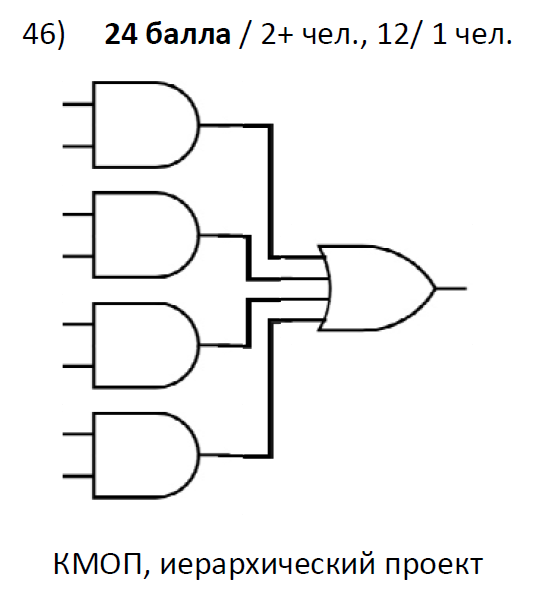
\includegraphics[width=0.4\linewidth]{image/schema_task}
	\caption{Схема задания}\label{img:schema_task}
\end{figure}

\section{Параметры схемы}

\begin{table}[H]	
	\begin{center}
	\begin{flushleft}
		\tablecaption{Топологические и геометрические нормы}
	\end{flushleft}
	\begin{tabular}{|l|l|l|}

		\hline
		Δ        & Минимальный топологический размер, мкм                                               & 0.25     \\ \hline
		& Минимальный размер стороны контактного окна                                          & 0.5Δ     \\ \hline
		& Минимальный размер фигуры в слое металла                                             & 0.5Δ     \\ \hline
		& Минимальное перекрытие металлом контактного окна                                     & 0.5Δ     \\ \hline
		& Минимальное расстояние от границ контактного   & 0.5Δ     \\ 
		& до границ контактируемой области   &     \\ \hline
		& Минимальное расстояние между фигурами в слое металла                                 & 0.5Δ     \\ \hline
		& Остальные топологические нормы                                                       & 0.5Δ     \\ \hline \hline
		
		$R_{sb}$         & Поверхностное сопротивление пассивной области базы, Ом                      & 300      \\ \hline
		$R_{sbb}$        & Поверхностное сопротивление активной области базы, Ом                       & 3000     \\ \hline
		$R_{se}$         & Поверхностное сопротивление области эмитера, Ом/□                           &     10     \\ \hline
		$C_{middle}$     & Ёмкость межсоединения, пФ                                                   &      10    \\ \hline
		$X_{jk}$         & глубина залегания p-n перехода базаколлектор, м                             & $1.1*10^{–6}$ \\ \hline
		$X_{je}$         & глубина залегания p-n перехода базаэмиттер, м                               & $0.5*10^{–6}$ \\ \hline
		$\omega_{epi}$   & толщина эпитаксиального слоя, м                                             & $4*10^{–6}  $ \\ \hline
		$X_{jn}$         & толщина скрытого n+ слоя, м                                                 & $1.0*10^{–6}$ \\ \hline
		$C_{pn0}$        & удельная ёмкость p-n-перехода, Ф/м2                                         & $3*10^{–3}  $ \\ \hline
		\hline
		
		Vdd      & Напряжение питания, В                                                       & $2.5     $ \\ \hline
		Смеж     & Ёмкость межсоединения, пФ                                                   & 10 \\ \hline
		tox      & Толщина подзатворного оксида, нм                                            & $6       $ \\ \hline
		μn       & Подвижность электронов, м2/(Вс)                                             & $0.0317  $ \\ \hline
		μp       & Подвижность дырок, м2/(Вс)                                                  & $0.0136  $ \\ \hline
		dпер     & Перекрытие затвором областей стока/истока, мкм                              & 0.1Δ    \\ \hline
		xj       & Глубина залегания p-n перехода нм                                           & 100 \\ 
		& исток-подложка и сток-подложка                                              & \\ \hline
		L        & длина канала, м                                                             & 1.0Δ     \\ \hline
	\end{tabular}
	\end{center}
\end{table}


\section{Работа транзисторов}

Рассмотрим 27 набор данных, который соответствует следующей бинарной последовательности: $0	0	0	1	1	0	1	1$. При подаче такого сигнала на схему на каждый элемент $AND$ будут поданы разные значения. Рассмотрим их.

\subsection{Первый элемент $AND$}

Элемент $AND$ изображён на \imref{img:schema_and}

\begin{figure}[H]
	\centering		
	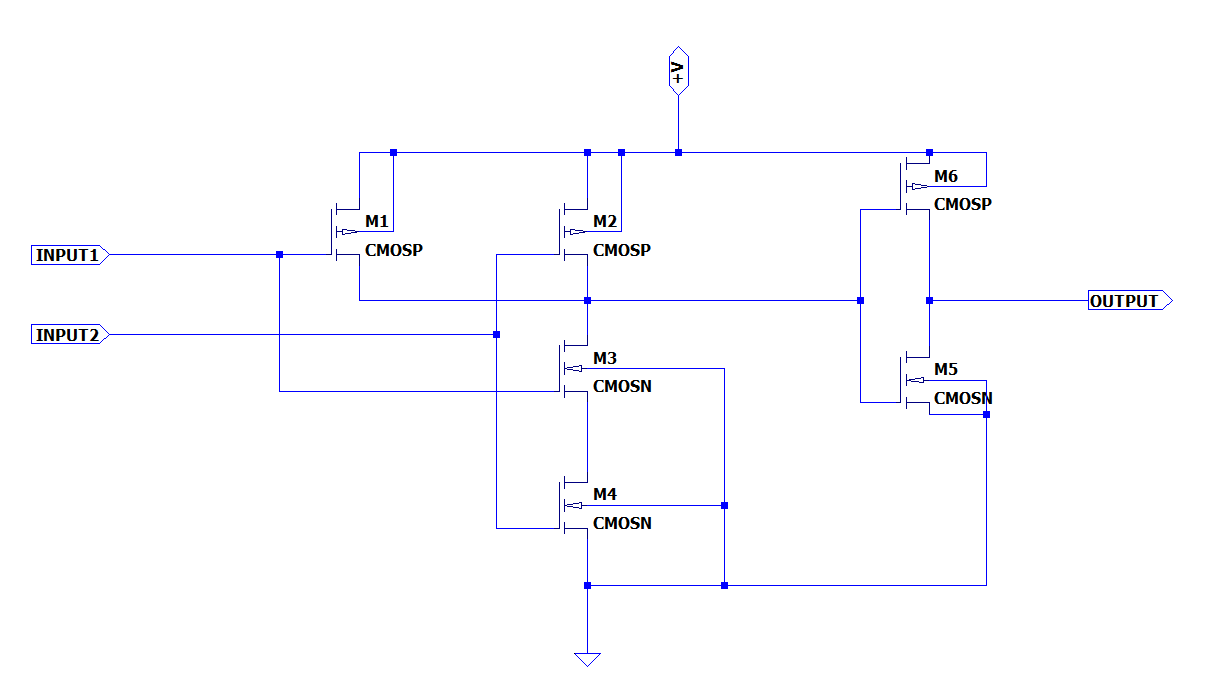
\includegraphics[width=\linewidth]{image/schema_and}
	\caption{Схема элемента И}\label{img:schema_and}
\end{figure}

На вход подаются значения $00$, транзисторы М1 и М2 остаются открытыми, а М3 и М4 закрытыми, на инвентор подаётся логическая 1, транзистор М6 закрыт, а М5 открыт, на выходе схемы получаем 0.

\subsection{Второй элемент $AND$}

На вход подаются значения $01$, транзисторы М1 и М4 остаются открытыми, а М3 и М2 закрытыми, на инвентор подаётся логическая 1, транзистор М6 закрыт, а М5 открыт, на выходе схемы получаем 0.

\subsection{Третий элемент $AND$}

На вход подаются значения $10$, транзисторы М2 и М3 остаются открытыми, а М1 и М4 закрытыми, на инвентор подаётся логическая 1, транзистор М6 закрыт, а М5 открыт, на выходе схемы получаем 0.

\subsection{Четвёртый элемент $AND$}

На вход подаются значения $11$, транзисторы М3 и М4 остаются открытыми, а М1 и М2 закрытыми, на инвентор подаётся логический 0, транзистор М6 открыт, а М5 закрыт, на выходе схемы получаем 1.

\subsection{Элемент $OR4$}

Элемент $OR4$ изображён на \imref{img:schema_or}

\begin{figure}[H]
	\centering		
	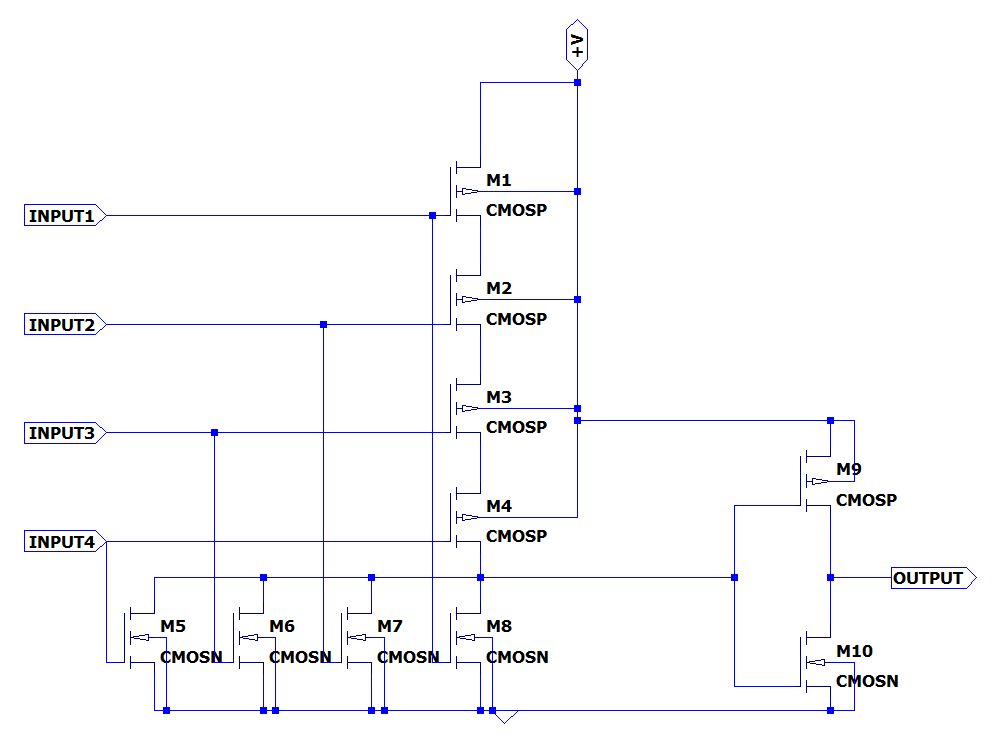
\includegraphics[width=\linewidth]{image/schema_or}
	\caption{Схема элемента 4-ИЛИ}\label{img:schema_or}
\end{figure}

На вход подаются значения $0001$, транзисторы М1, М2, М3 и М5 остаются открытыми, а М4, М6, М7 и М8	 закрытыми, на инвентор подаётся логический 0, транзистор М9 открыт, а М10 закрыт, на выходе схемы получаем 1.

TODO описать все комбинаиции для И-4
\section{Тут идёт кусок теории}

\section{Расчёт параметров схемы}

Для удобства проектирования схемы в LTSpice были созданы переменные, некоторые из которых зависят от исходных

$ Vol = 2.5V  $ -- Напряжение питания

$ un = 0.0317 $ -- Подвижность электронов

$ up = 0.0136 $ -- Подвижность дырок

$ LChan=0.25u $ -- Длина канала

$ WtoL=8 $ -- Выбор отношения ширины канала к длине

$ Depth=3.75u $ -- Глубина канала по построению

$ WN=WtoL * LChan $ -- Ширина канала для NMOPT

$ WP= \frac{un}{up} * WtoL* LChan $ -- Ширина канала для PMOPT

$ ASN=WN * Depth $ -- Площадь стока для NMOPT

$ ADN= ASN $-- Площадь истока для NMOPT

$ ASP=WP * Depth$ -- Площадь стока для PMOPT

$ ADP=ASP $ -- Площадь стока для PMOPT

$ PSN=2 * WN + Depth $ -- Периметр истока для NMOPT

$ PDN=2 * WN + Depth $ -- Периметр стока для NMOPT

$ PSP=2 * WP + Depth $ -- Периметр истока для PMOPT

$ PDP=2 * WP + Depth $ -- Периметр стока для PMOPT


\section{Вид сверху и слайсы}

\section{Spice calculator}

Схемы элементов представлены на \imref{img:schema_and} и \imref{img:schema_or}

\subsection{Таблица истинности}

\begin{figure}[H]
	\centering		
	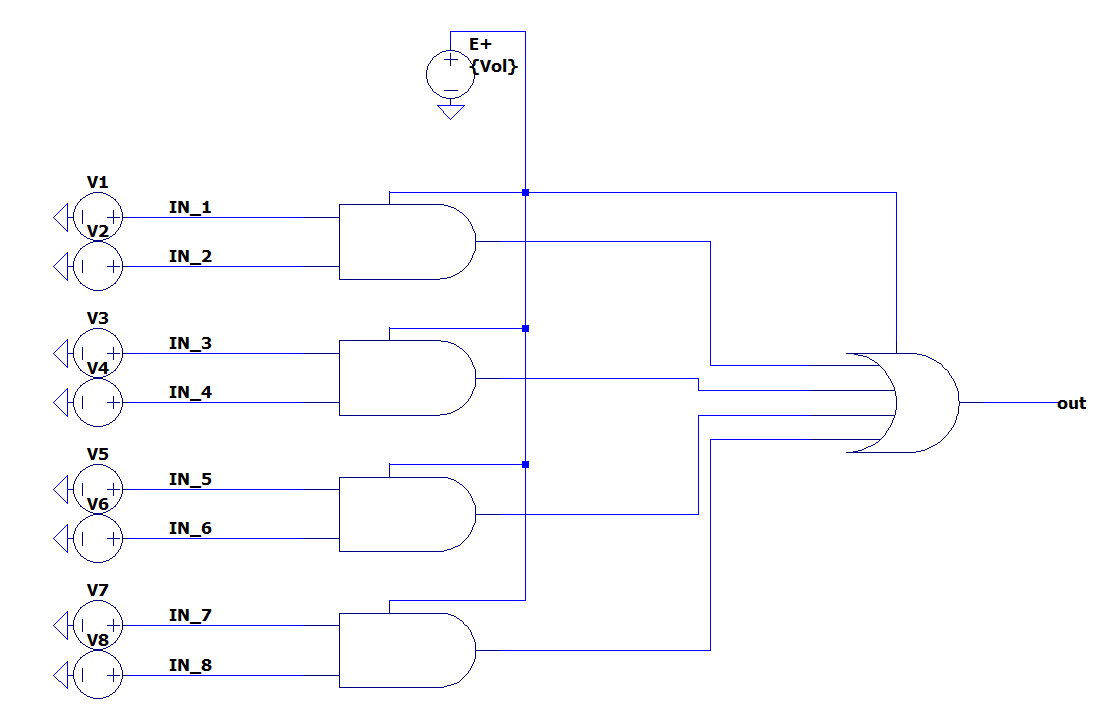
\includegraphics[width=\linewidth]{image/schema_all}
	\caption{Схема для проверки таблицы истинности}\label{img:schema_all}
\end{figure}


\begin{figure}[H]
	\centering		
	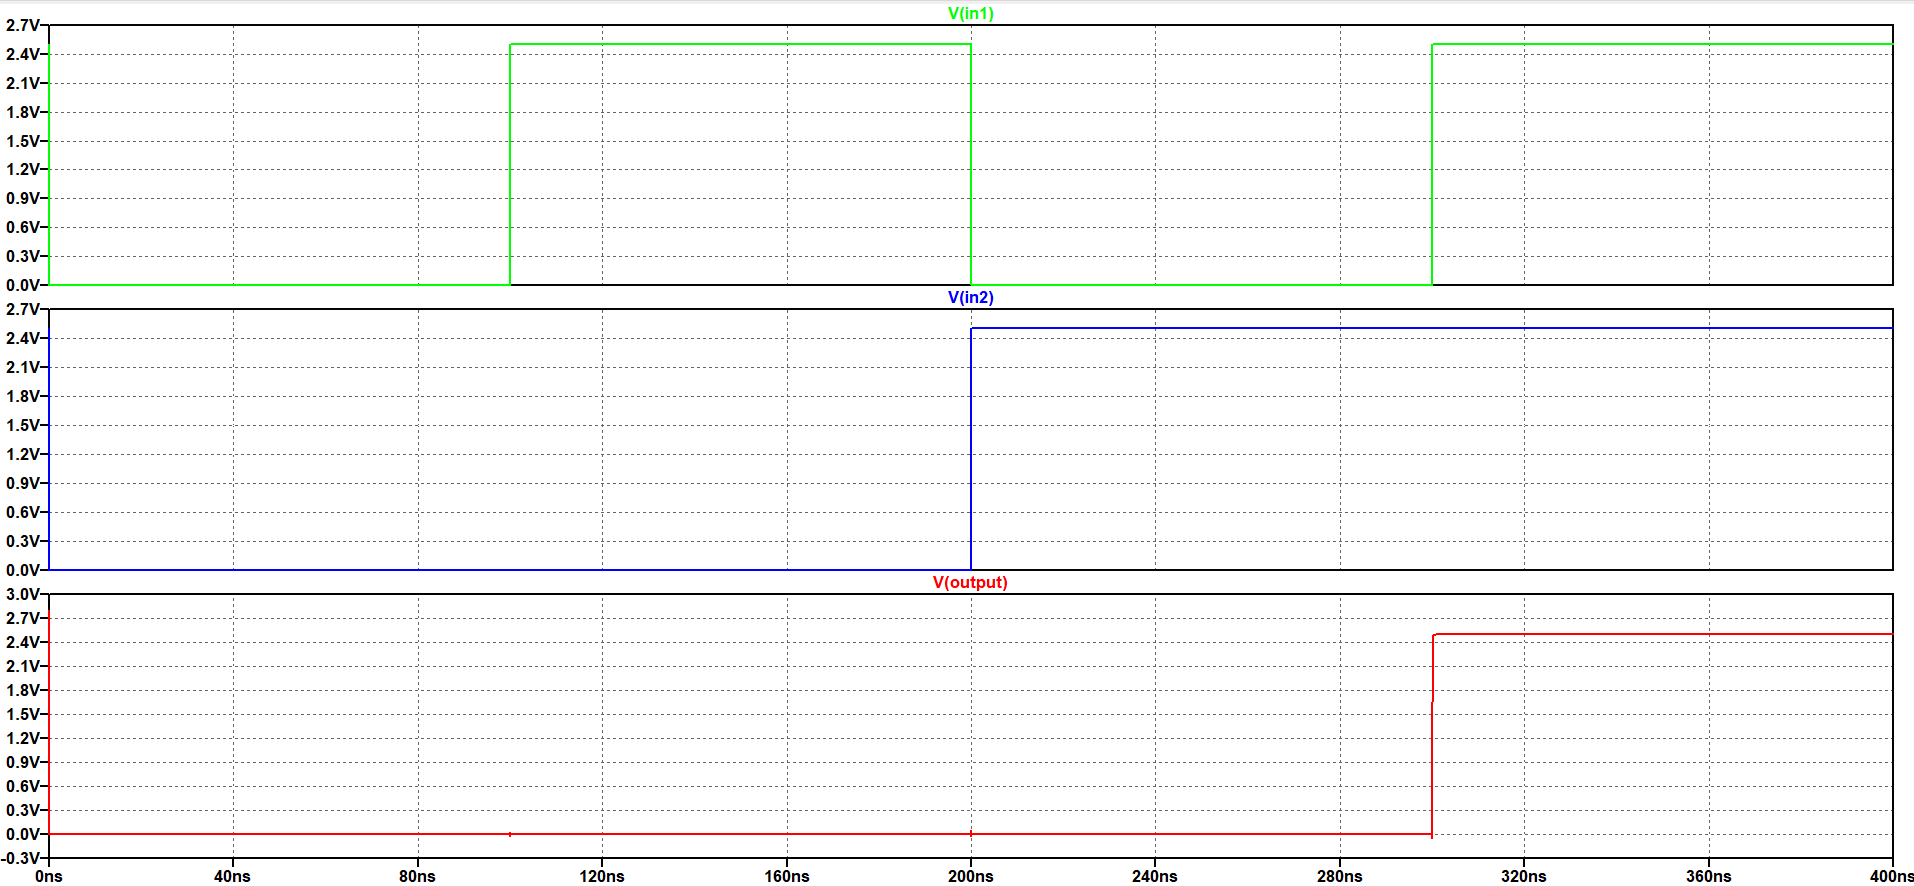
\includegraphics[width=\linewidth]{image/spice_and_bin}
	\caption{Таблица истинности для элемента И}\label{img:spice_and_bin}
\end{figure}


\begin{figure}[H]
	\centering		
	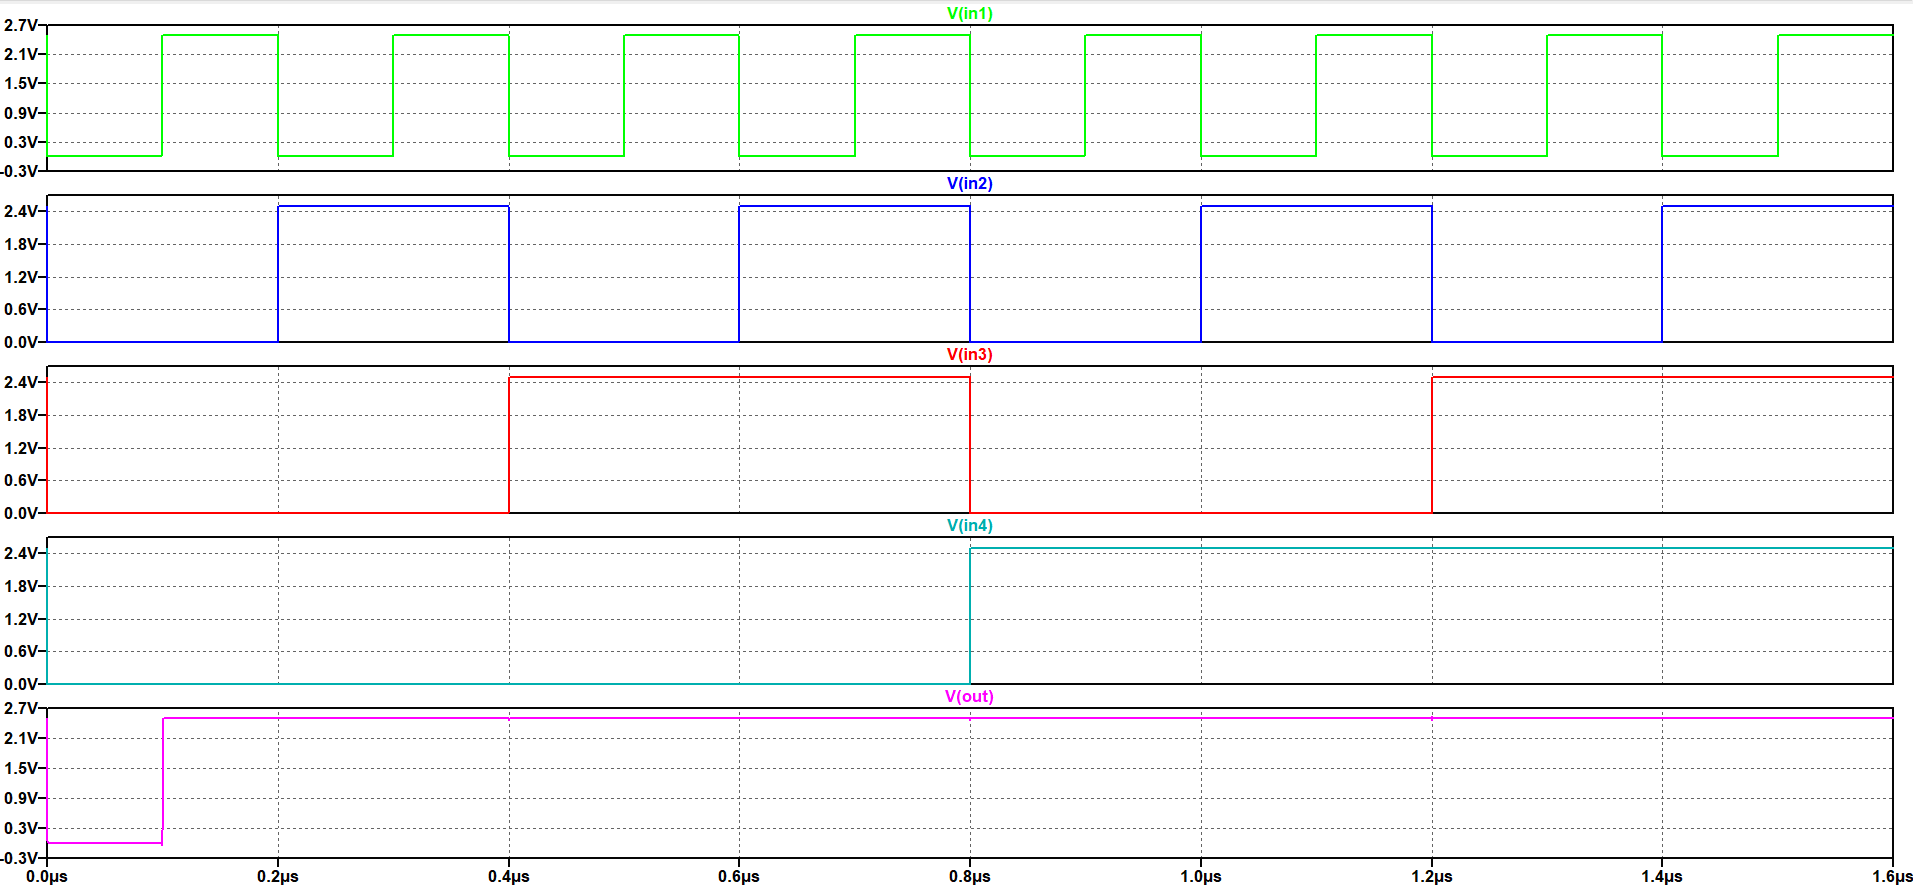
\includegraphics[width=\linewidth]{image/spice_or_bin}
	\caption{Таблица истинности для элемента-ИЛИ }\label{img:spice_or_bin}
\end{figure}

\begin{figure}[H]
	\centering		
	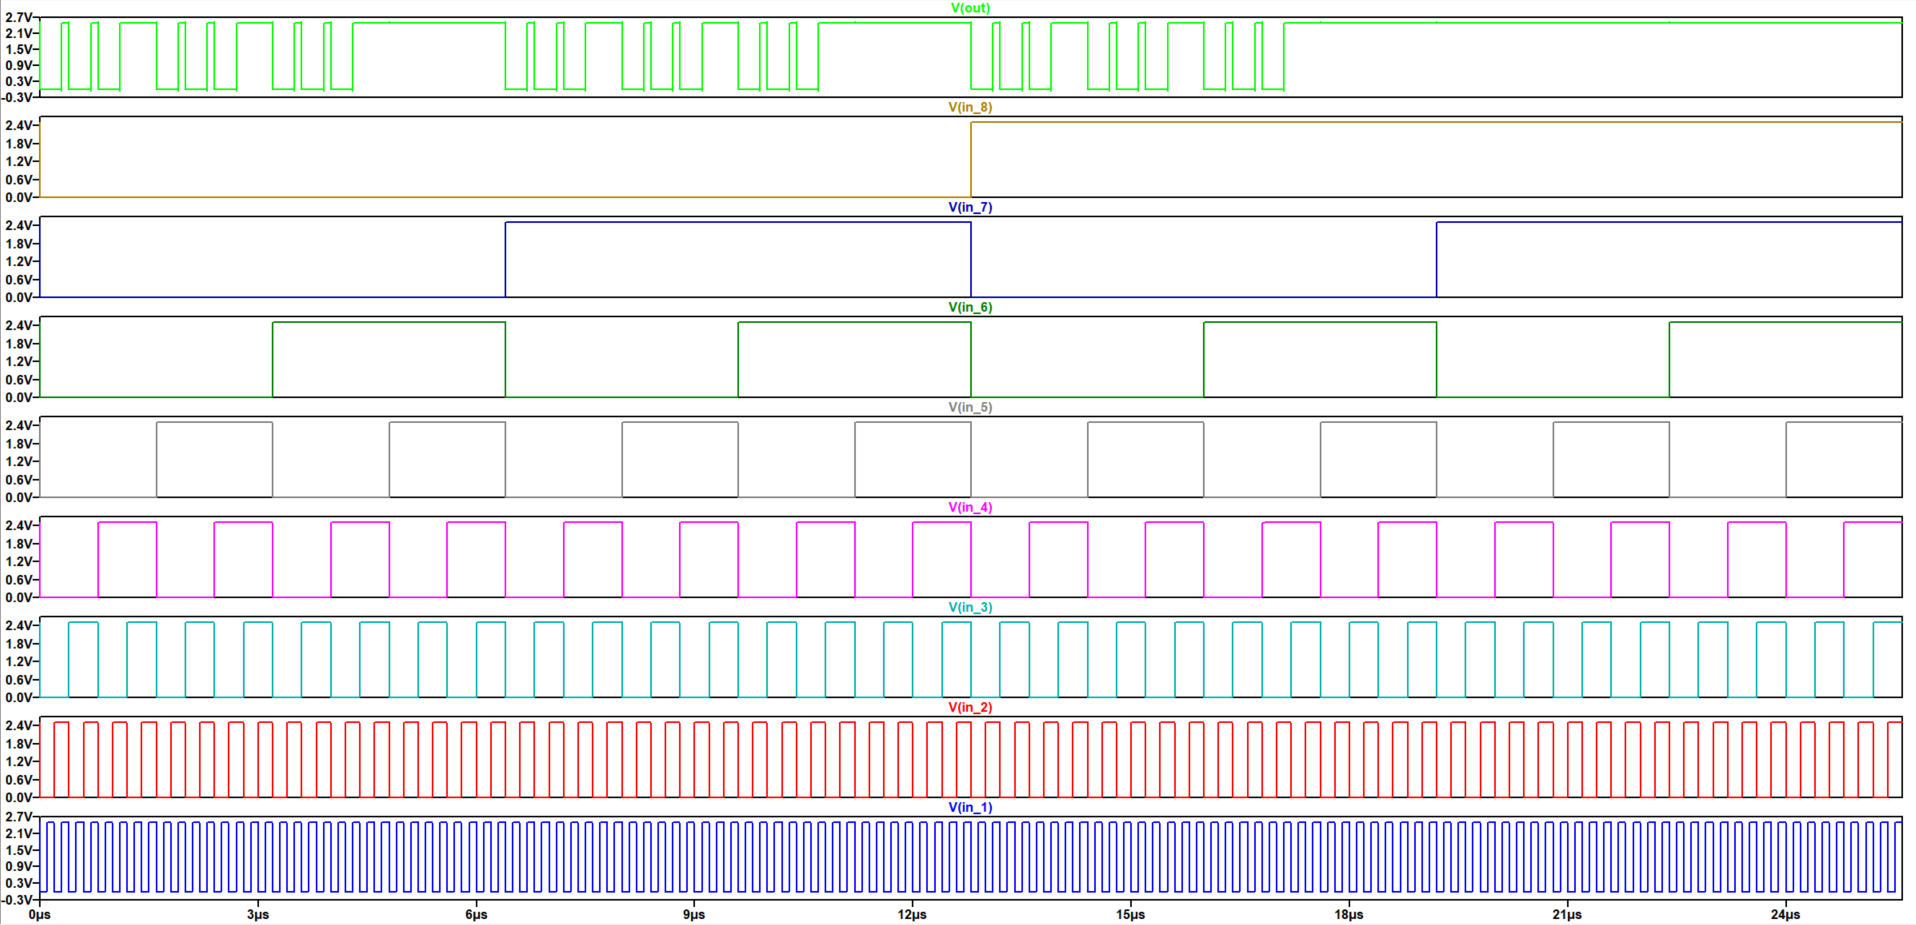
\includegraphics[width=\linewidth]{image/spice_bin}
	\caption{Таблица истинности всей схемы}\label{img:spice_bin}
\end{figure}

\subsection{Анализ статических характеристик}

\begin{figure}[H]
	\centering		
	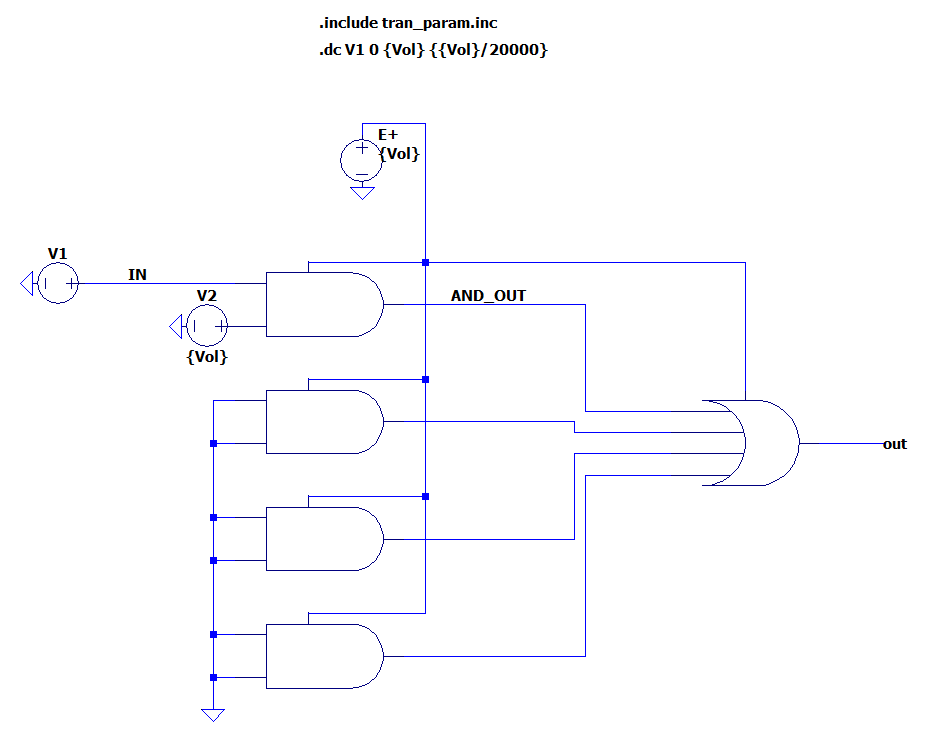
\includegraphics[width=\linewidth]{image/dc_schema}
	\caption{Схема для расчёта статических характеристик}\label{img:dc_schema}
\end{figure}

\begin{figure}[H]
	\centering		
	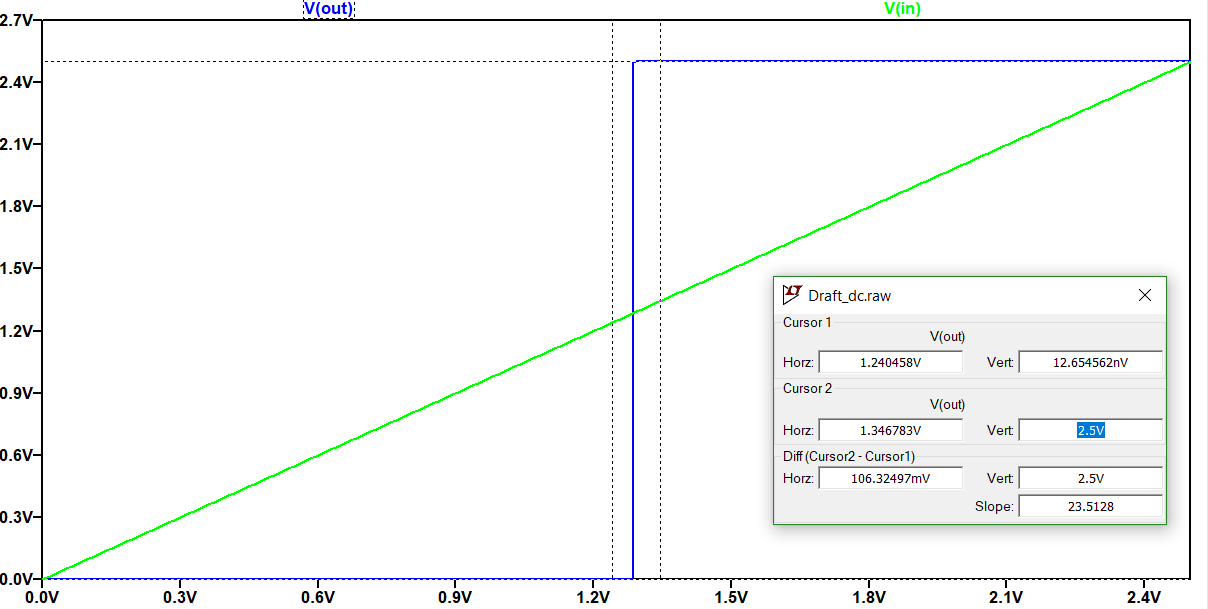
\includegraphics[width=\linewidth]{image/dc_V_01}
	\caption{Передаточная характеристика схемы}\label{img:dc_V_01}
\end{figure}

\begin{figure}[H]
	\centering		
	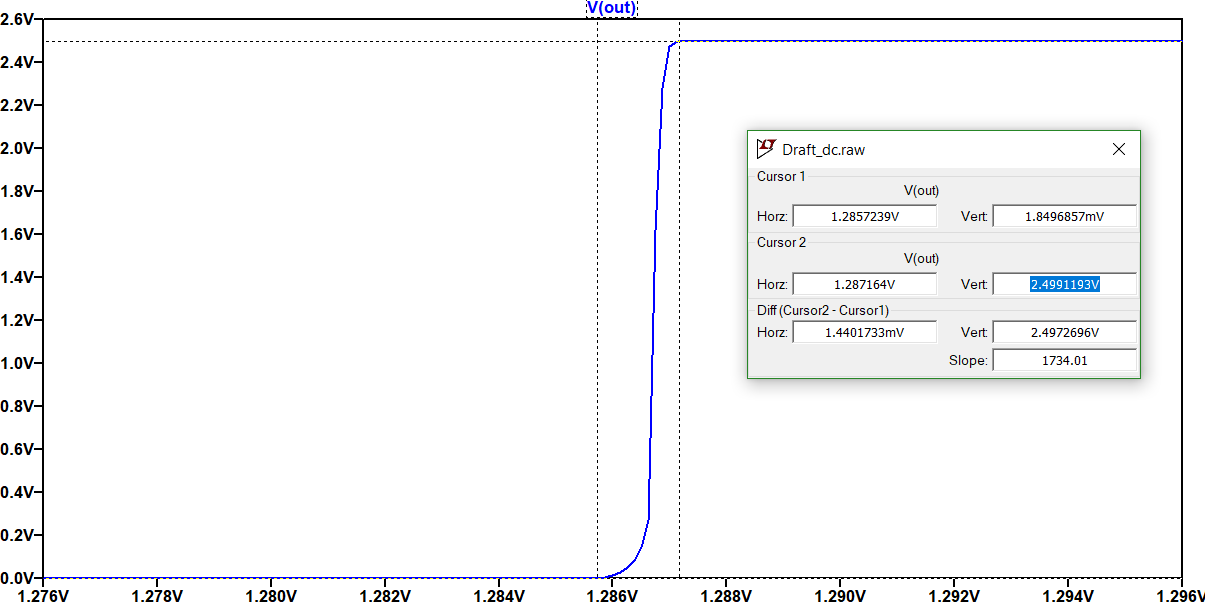
\includegraphics[width=\linewidth]{image/dc_V}
	\caption{Увеличенная область перехода}\label{img:dc_V}
\end{figure}

\begin{figure}[H]
	\centering		
	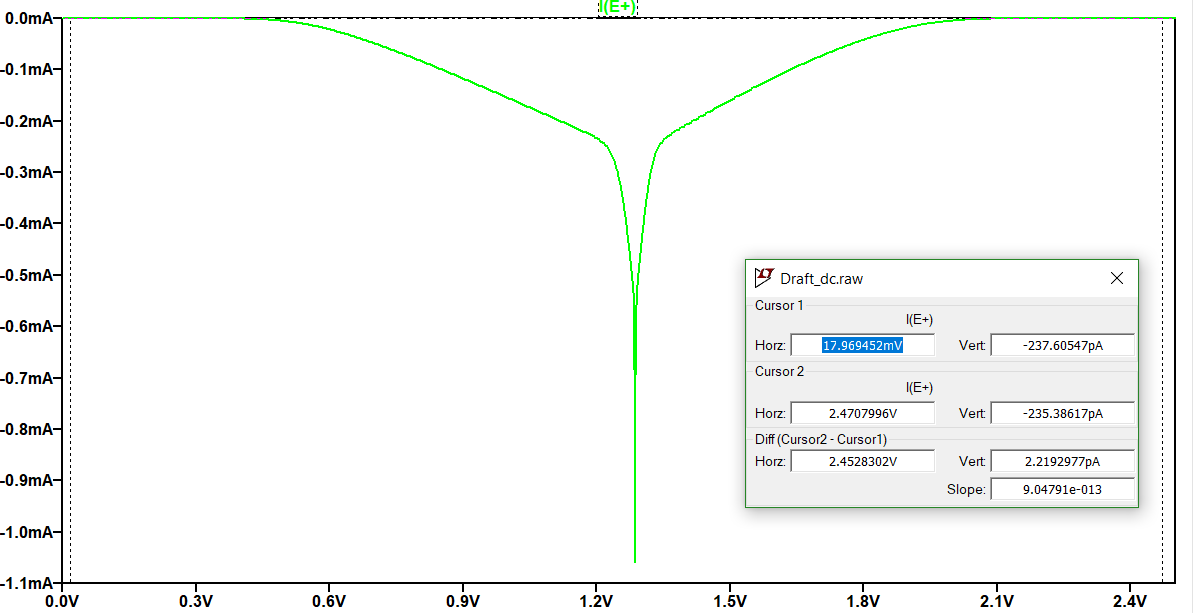
\includegraphics[width=\linewidth]{image/dc_I}
	\caption{Потребляемый ток включённой и выключенной схемы}\label{img:dc_I}
\end{figure}

\begin{figure}[H]
	\centering		
	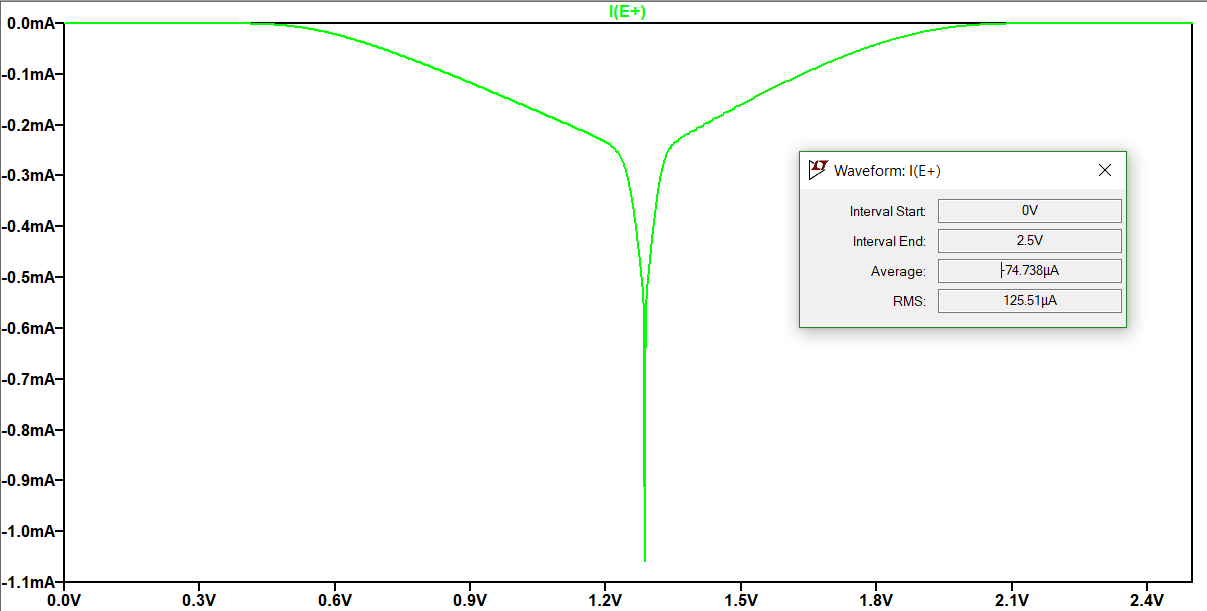
\includegraphics[width=\linewidth]{image/dc_I_avg}
	\caption{Средний ток}\label{img:dc_I_avg}
\end{figure}

Данные измерений и расчётов:

$U_{log}^0 = 12 nV \approx 0$

$U_{log}^1 = 2.5 V$

$U_{log} = 2.5 V$

$I_0 \approx 0 A $

$I_1 \approx 0 A $

$I_{avg} = -74 mkA $

$V_p^0 = 1.2857V$

$V_p^1 = 1.2871V$

$U_{err}^{+} = 1.2857V - 12nV \approx 1.29V $

$U_{err}^{-} = 2.5V - 1.2871 \approx 1.21V $

$P_{static} = \frac{2.5V \times (0 + 0)}{2} = 0$

\subsection{Анализ динамических характеристик}

\begin{figure}[H]
	\centering
	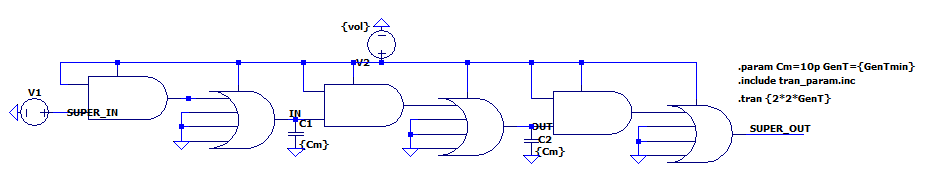
\includegraphics[width=0.7\linewidth]{image/dyn_shema_min}
	\caption{Схема расчета динамических характеристик}
	\label{fig:dynshema}
\end{figure}

\begin{figure}[H]
	\centering
	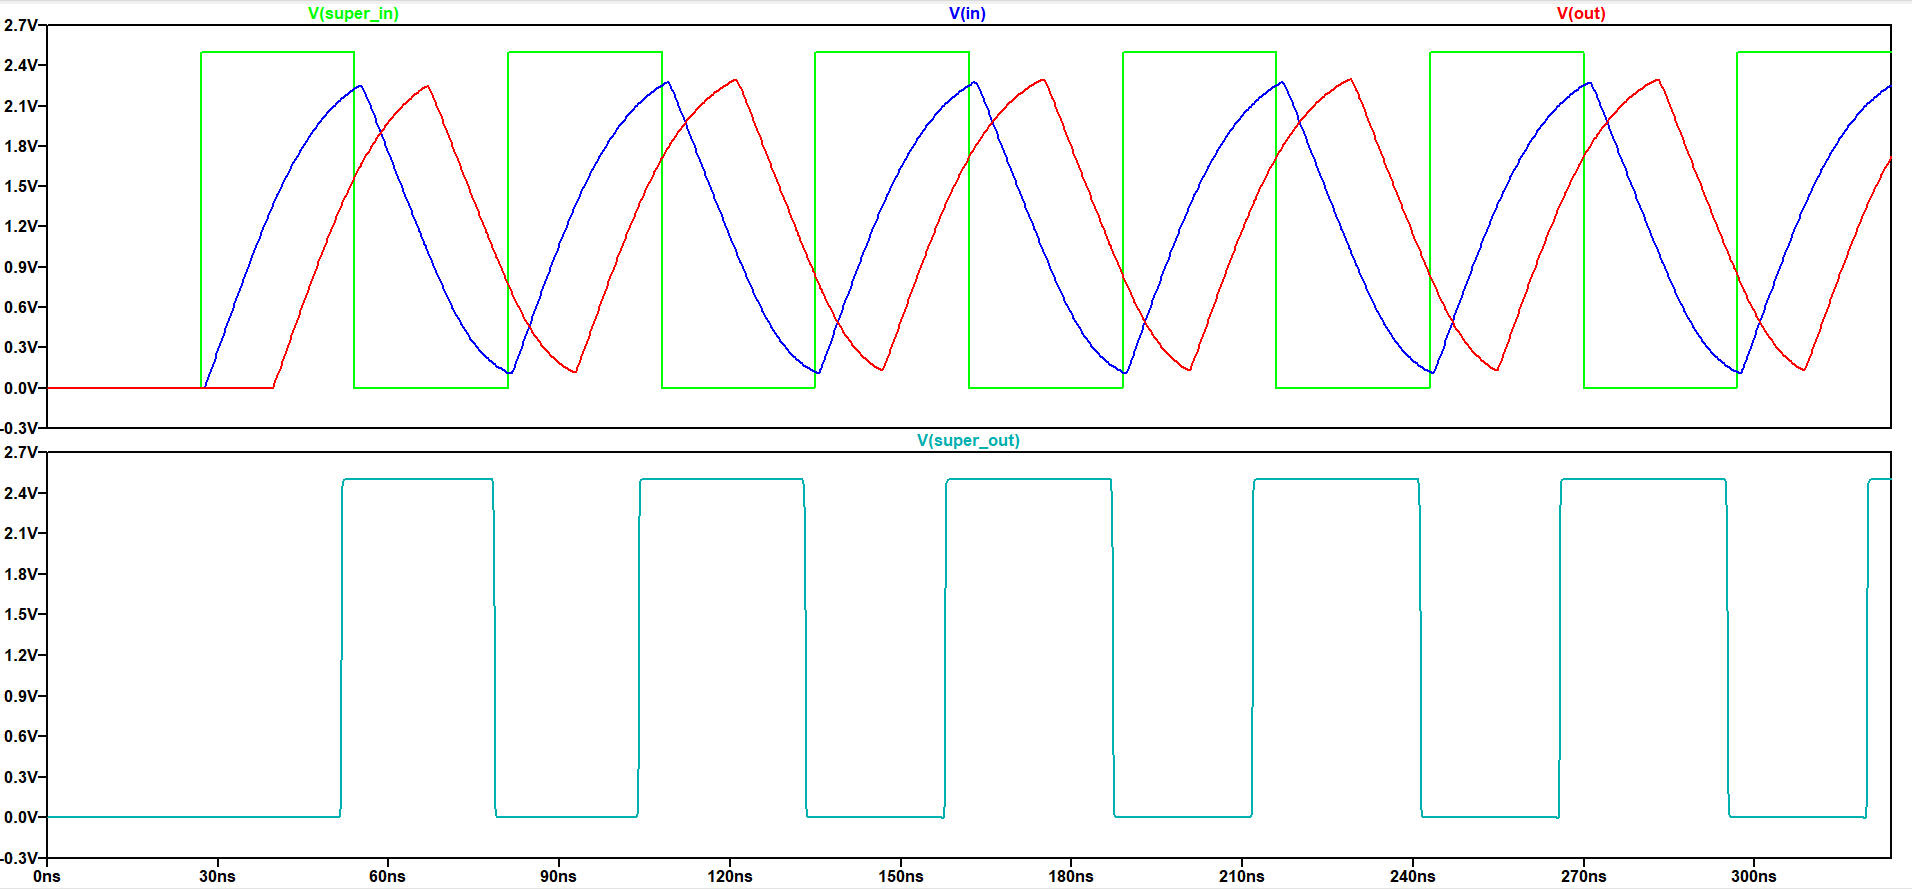
\includegraphics[width=\linewidth]{image/dyn_max_freq}
	\caption{}
	\label{fig:dyn_max_freq}
\end{figure}

\begin{figure}[H]
	\centering
	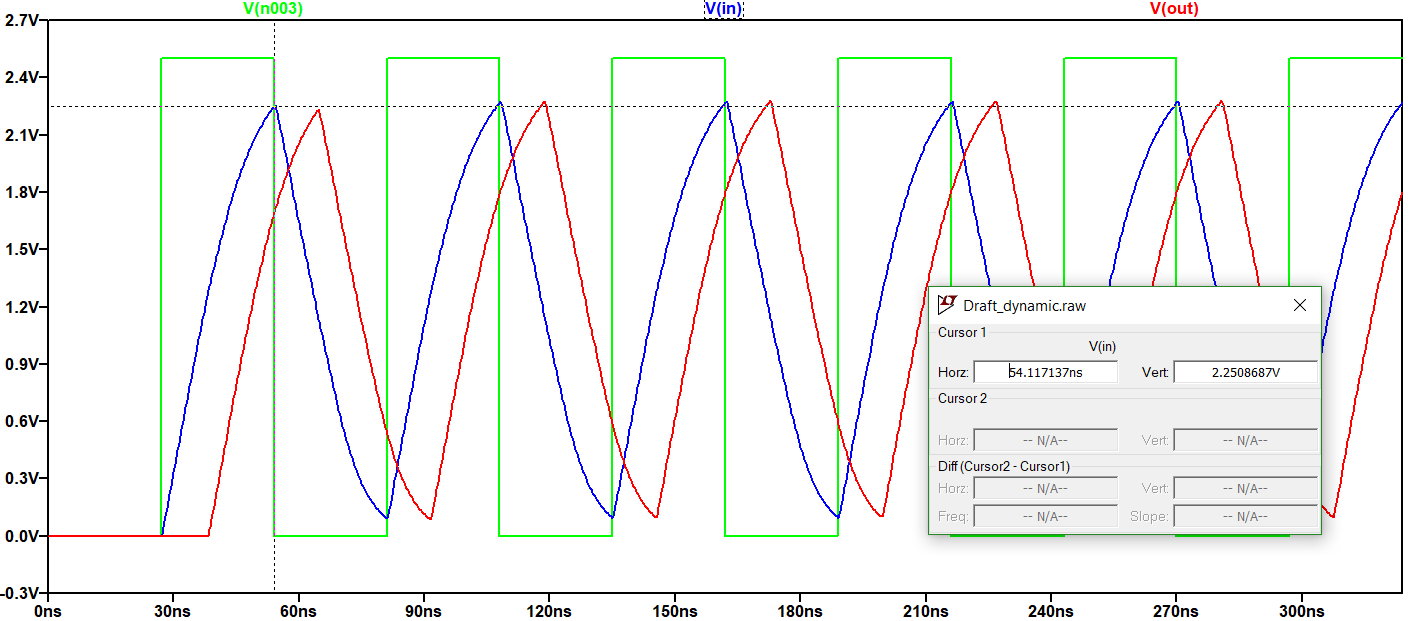
\includegraphics[width=\linewidth]{image/dyn_max_volt}
	\caption{}
	\label{fig:dyn_max_volt}
\end{figure}

$$T(f_{max}) = 27ns$$
$$f_{max} = \dfrac{1}{T_{max}} \approx 37.037 MHz$$

\begin{figure}[H]
	\centering
	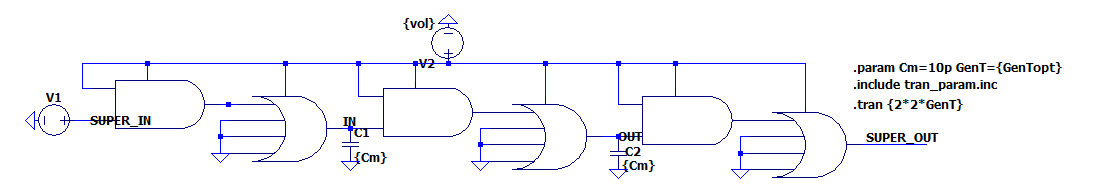
\includegraphics[width=0.7\linewidth]{image/dyn_shema_opt}
	\caption{}
	\label{fig:dynshemamin}
\end{figure}

\begin{figure}[H]
	\centering
	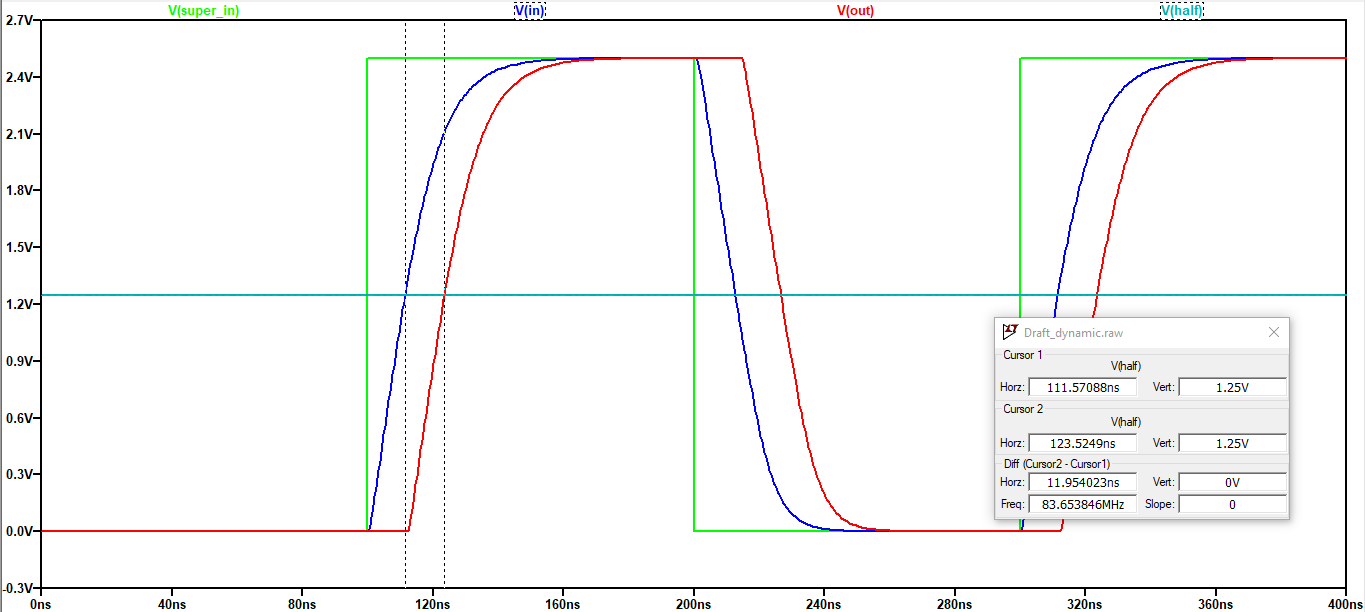
\includegraphics[width=\linewidth]{image/dyn_opt_zad01}
	\caption{}
	\label{fig:dynoptzad01}
\end{figure}


\begin{figure}[H]
	\centering
	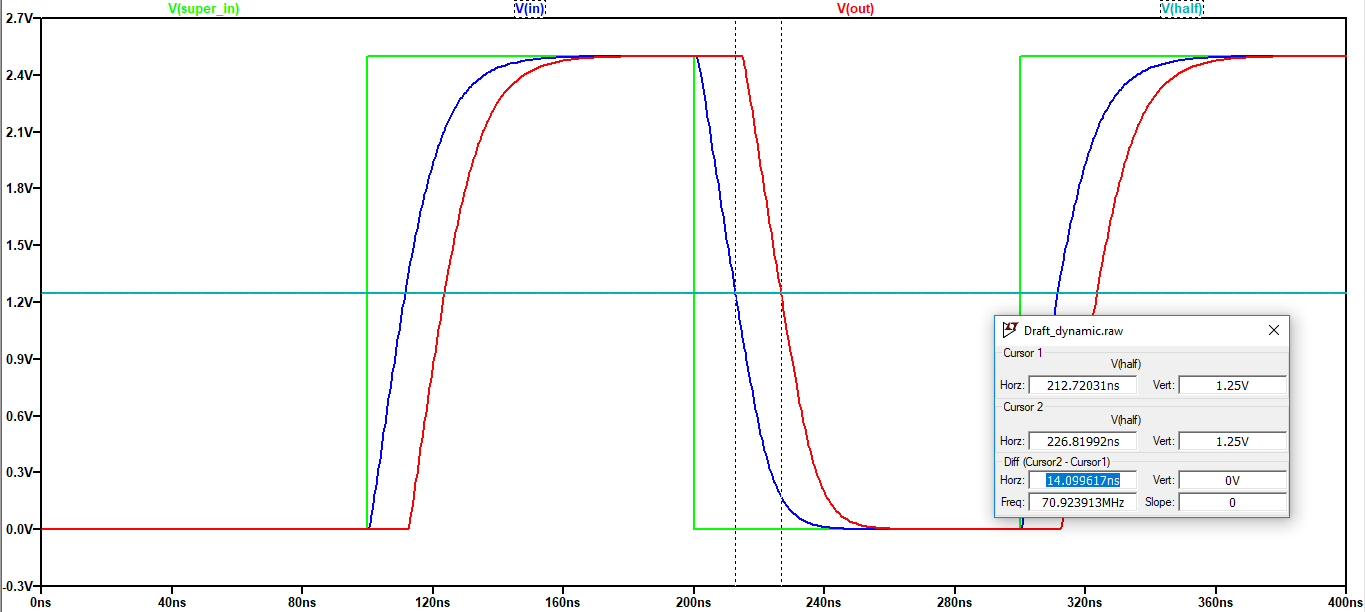
\includegraphics[width=\linewidth]{image/dyn_opt_zad10}
	\caption{}
	\label{fig:dynoptzad10}
\end{figure}

$$t_{z}^{01} = 12ns$$
$$t_{z}^{10} = 14ns$$
$$t_{z} = \dfrac{t_{z}^{01} + t_{z}^{10}}{2} = 13ns$$

\begin{figure}[H]
	\centering
	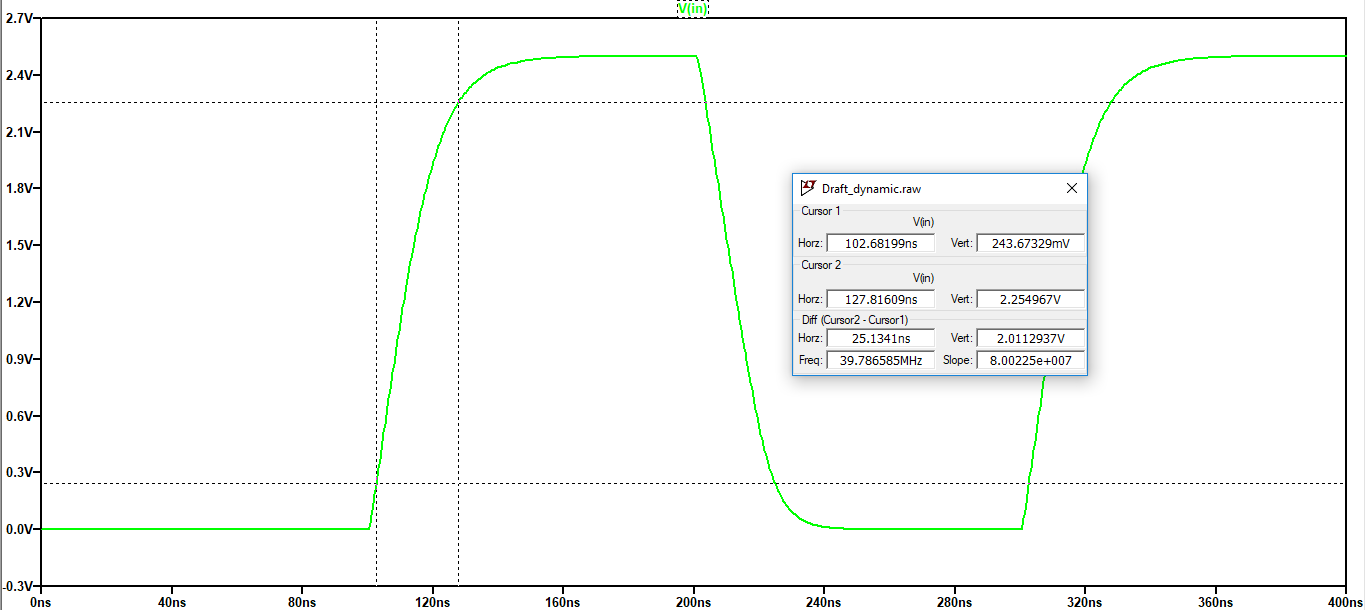
\includegraphics[width=\linewidth]{image/dyn_opt_f01}
	\caption{}
	\label{fig:dynoptf01}
\end{figure}

\begin{figure}[H]
	\centering
	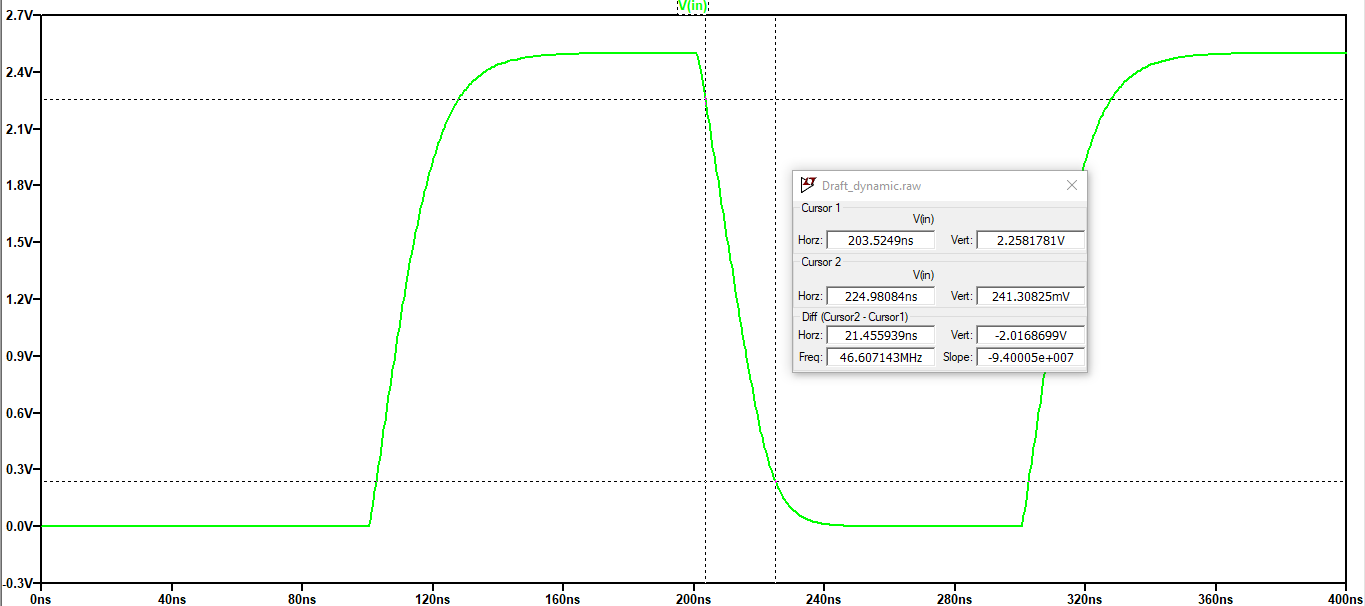
\includegraphics[width=\linewidth]{image/dyn_opt_f10}
	\caption{}
	\label{fig:dynoptf10}
\end{figure}

$$$t_{f}^{01} = 25ns$
$$$t_{f}^{10} = 21ns$
$$f_{p} = \dfrac{1}{T} = $$




\section{Топология}

\begin{landscape}
\begin{figure}[H]
	\centering		
	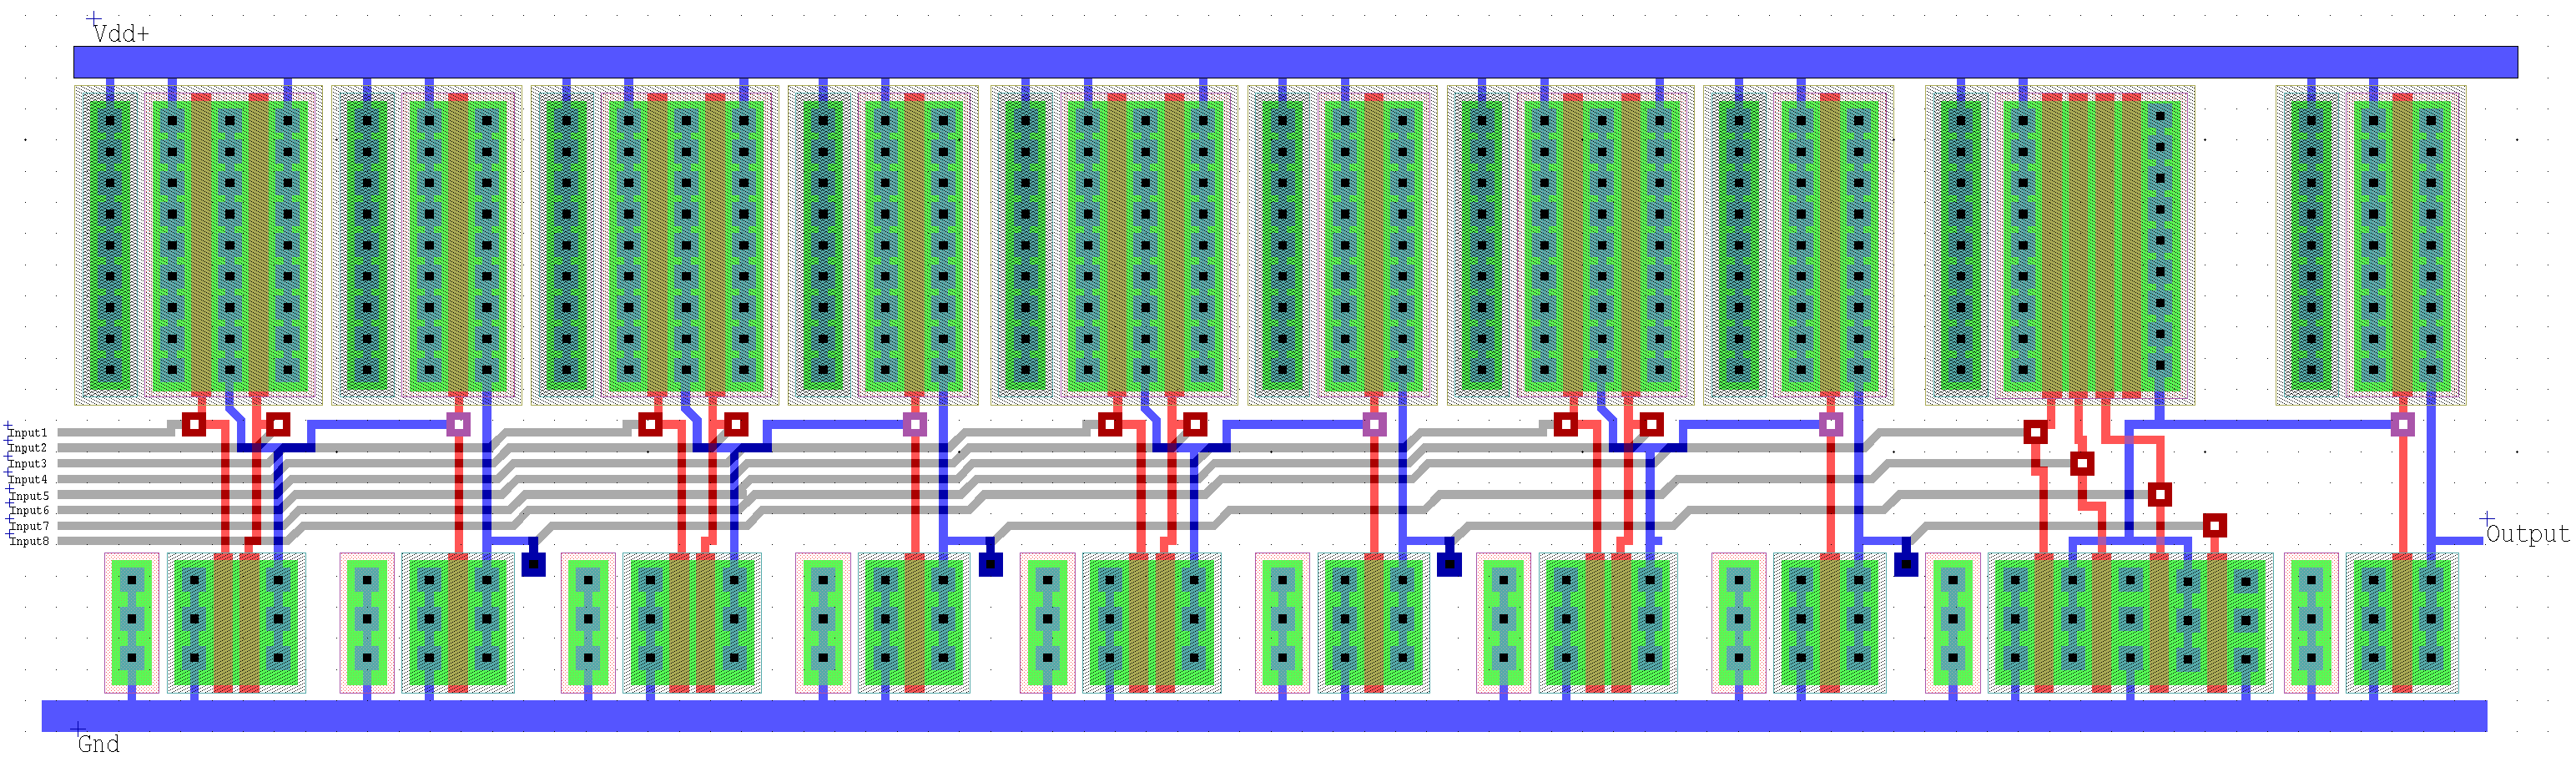
\includegraphics[width=\linewidth]{image/ledit_schema}
	\caption{Топология}\label{img:ledit_schema}
\end{figure}
\end{landscape}

\section{Вывод}

Всё тлен

\end{document} % конец документа